\documentclass{article}

\usepackage[final]{neurips_2026}

\usepackage[utf8]{inputenc}
\usepackage[T1]{fontenc}
\usepackage{hyperref}
\usepackage{url}
\usepackage{booktabs}
\usepackage{amsmath}
\usepackage{amsfonts}
\usepackage{nicefrac}
\usepackage{microtype}
\usepackage{xcolor}
\usepackage{graphicx}

\makeatletter
\def\@noticestring{}
\makeatother

\title{HW1 Report: A Three-Layer MLP from Scratch for EuroSAT RGB Land Cover Classification}

\author{%
  Cheng Zihao\\
  School of Data Science \\
  \texttt{25210980152@m.fudan.edu.cn}
}

\begin{document}

\maketitle

\begin{abstract}
This report presents Homework 1 on building a three-layer multilayer perceptron (MLP) from scratch for EuroSAT RGB land cover classification. The entire training pipeline was implemented with NumPy, including forward propagation, manual backpropagation, softmax cross-entropy, stochastic gradient descent (SGD), learning-rate decay, weight decay, checkpoint selection, evaluation, staged hyperparameter search, and visualization. No automatic differentiation framework such as PyTorch, TensorFlow, or JAX was used. In the final experiment, a two-stage search strategy was applied: a 54-trial coarse grid search first identified a promising region of the hyperparameter space, and a 27-trial fine grid search then refined the configuration around the coarse optimum. The coarse stage systematically compared ReLU, Tanh, and Sigmoid, and showed a clear advantage for ReLU. The final model, trained with the best fine-search configuration, reached a best validation accuracy of \(0.6788\) at epoch 30 and a test accuracy of \(0.6780\). The report further analyzes the search strategy, result tables, confusion matrix, first-layer weights, and representative failure cases.
\end{abstract}

\section{Introduction}

The goal of this homework is to implement an image classifier for the EuroSAT RGB dataset using a three-layer MLP trained entirely from scratch. The task is multi-class land cover classification with 10 categories: AnnualCrop, Forest, HerbaceousVegetation, Highway, Industrial, Pasture, PermanentCrop, Residential, River, and SeaLake.

The main technical constraint of the assignment is that the learning procedure must not rely on automatic differentiation. Therefore, all trainable layers, activation functions, gradients, and optimization steps were implemented manually in NumPy. The completed project includes modular components for data loading, preprocessing, model definition, training, hyperparameter search, testing, and visualization under \texttt{code/}, while all generated artifacts are saved under \texttt{results/}.

\section{Dataset and Preprocessing}

The dataset used in this homework is \texttt{EuroSAT\_RGB/}, organized as one subdirectory per class. Inspection of the local dataset shows that the raw RGB images are consistently \(64 \times 64\). The implemented loader reads these images, resizes them to a fixed spatial resolution for training, converts them to floating-point arrays, and normalizes pixel values to \([0, 1]\).

In the main experiment, the raw \(64 \times 64\) images were resized to \(32 \times 32\), resulting in an input dimensionality of \(32 \times 32 \times 3 = 3072\) after flattening. A fixed random seed of 42 was used throughout the pipeline for reproducibility. The dataset was split in a stratified manner into training, validation, and test subsets with ratios \(70\%\), \(15\%\), and \(15\%\), respectively. The resulting split sizes are shown in Table~\ref{tab:data_split}.

Channel-wise standardization was computed from the training split only and then applied to all subsets. Mini-batch iteration was implemented in NumPy with shuffling enabled for training.

The resize step is a practical design choice rather than a claim that the original data are low resolution. For a fully connected MLP, using the raw \(64 \times 64\) images would increase the flattened input dimensionality from 3072 to 12288 and would enlarge the first-layer parameter count by a factor of four. This would substantially increase training cost, make hyperparameter search less feasible, and raise the risk of overfitting for a dense architecture that does not explicitly exploit local spatial structure. Resizing to \(32 \times 32\) inevitably removes some fine texture information, but it provides a better trade-off between computational cost, numerical stability, and classification performance for a from-scratch NumPy MLP.

Table~\ref{tab:class_distribution} summarizes the class distribution directly read from the dataset folders. The dataset is nearly balanced, although Highway, Industrial, PermanentCrop, River, and Pasture contain fewer images than AnnualCrop, Forest, Residential, and SeaLake. This mild imbalance is useful to mention in the report because it partially explains why some categories are slightly harder than others even before model-specific limitations are considered.

\begin{table}[t]
  \caption{Dataset split and input configuration used in the final training pipeline. The raw images are \(64 \times 64\), while the MLP input is resized to \(32 \times 32\).}
  \label{tab:data_split}
  \centering
  \begin{tabular}{lr}
    \toprule
    Item & Value \\
    \midrule
    Number of classes & 10 \\
    Raw image size & \(64 \times 64 \times 3\) \\
    Training input size & \(32 \times 32 \times 3\) \\
    Flattened input dimension & 3072 \\
    Training samples & 18{,}900 \\
    Validation samples & 4{,}050 \\
    Test samples & 4{,}050 \\
    Split ratio & 70 / 15 / 15 \\
    Random seed & 42 \\
    \bottomrule
  \end{tabular}
\end{table}

\begin{table}[t]
  \caption{Class distribution in the EuroSAT RGB dataset, read from the local \texttt{EuroSAT\_RGB/} directory.}
  \label{tab:class_distribution}
  \centering
  \small
  \begin{tabular}{lr}
    \toprule
    Class & Number of Images \\
    \midrule
    AnnualCrop & 3{,}000 \\
    Forest & 3{,}000 \\
    HerbaceousVegetation & 3{,}000 \\
    Highway & 2{,}500 \\
    Industrial & 2{,}500 \\
    Pasture & 2{,}000 \\
    PermanentCrop & 2{,}500 \\
    Residential & 3{,}000 \\
    River & 2{,}500 \\
    SeaLake & 3{,}000 \\
    \midrule
    Total & 27{,}000 \\
    \bottomrule
  \end{tabular}
\end{table}

\section{Model Architecture}

The classifier is a three-layer MLP with the following structure:
\[
\text{input} \rightarrow \text{hidden}_1 \rightarrow \text{activation} \rightarrow \text{hidden}_2 \rightarrow \text{activation} \rightarrow \text{output}.
\]

For the final main training run, the network used hidden dimensions 768 and 384 with ReLU activation in both hidden layers. The output layer produced logits for the 10 land cover classes. The implementation supports ReLU, Tanh, and Sigmoid activations. In the updated systematic search, all three activations were considered in the coarse stage, after which the fine stage focused only on ReLU because it was the strongest activation family in the broader comparison.

Each linear layer stores its own parameters and intermediate cache for backpropagation. The backward pass explicitly computes gradients for weights and biases, and the optimizer updates parameters using SGD. This design follows the assignment requirement that the training process be implemented without any automatic differentiation engine.

\section{Training Method}

The training objective is softmax cross-entropy with \(L_2\) regularization applied to the weight matrices. The optimization pipeline is shared by both the hyperparameter-search runs and the final full training run. In every experiment, the implementation uses mini-batch SGD, explicit manual backpropagation, learning-rate decay, and model selection by validation accuracy.

For each candidate configuration evaluated during search, the code records training loss, validation loss, validation accuracy, and learning rate at every epoch. The checkpoint with the best validation accuracy is saved automatically to \texttt{results/checkpoints/}. After the hyperparameter search determines the best configuration, the same training procedure is reused for the final 30-epoch run.

The final full-training configuration, selected after the two-stage search, is summarized below:

\begin{itemize}
\item batch size: 128
\item epochs: 30
\item hidden dimensions: 768 and 384
\item activation: ReLU
\item initial learning rate: 0.06
\item learning-rate decay: 0.95 per epoch
\item minimum learning rate: \(10^{-4}\)
\item weight decay: \(10^{-5}\)
\end{itemize}

\section{Hyperparameter Search Strategy}

To make the hyperparameter study more systematic, the final experiment used a two-stage grid-search strategy rather than a single short random search. The goal was to first identify a promising region of the search space and then refine the candidate configuration before running the full 30-epoch training used for the final model.

\paragraph{Stage 1: coarse search.}
The coarse search explored a relatively broad grid over four hyperparameters:
\begin{itemize}
\item learning rate: \(\{0.03, 0.01, 0.003\}\)
\item hidden dimension of the first layer: \(\{128, 256, 512\}\)
\item weight decay: \(\{0, 10^{-4}\}\)
\item activation: \{\texttt{relu}, \texttt{tanh}, \texttt{sigmoid}\}
\end{itemize}
The second hidden dimension was set to half of the first hidden dimension. This coarse stage evaluated \(3 \times 3 \times 2 \times 3 = 54\) configurations, each trained for 10 epochs. The best coarse-search configuration was \texttt{ReLU}, learning rate \(0.03\), hidden dimensions \(512\) and \(256\), and zero weight decay, with a best validation accuracy of \(0.6600\). Sigmoid was clearly weaker than both ReLU and Tanh in this broader comparison, so it was not retained for the fine search.

\paragraph{Stage 2: fine search.}
The fine search then focused on the neighborhood of the coarse optimum. Since the coarse search strongly favored ReLU and larger hidden widths, while Sigmoid performed substantially worse and Tanh remained consistently behind ReLU, the fine stage fixed the activation to ReLU and searched:
\begin{itemize}
\item learning rate: \(\{0.015, 0.03, 0.06\}\)
\item hidden dimension of the first layer: \(\{256, 512, 768\}\)
\item weight decay: \(\{0, 10^{-5}, 10^{-4}\}\)
\item activation: \{\texttt{relu}\}
\end{itemize}
This produced \(3 \times 3 \times 3 \times 1 = 27\) configurations, each trained for 15 epochs. The best fine-search configuration used learning rate \(0.06\), hidden dimensions \(768\) and \(384\), weight decay \(10^{-5}\), and ReLU activation, reaching a best validation accuracy of \(0.6711\).

This staged strategy is the main practical contribution of the final experiment: instead of treating hyperparameter search as a small sanity check, it was turned into a structured procedure that first covered the broader design space and then refined the most promising region.

\begin{table}[ht]
  \caption{Summary of the two-stage hyperparameter search strategy and the best configuration found at each stage.}
  \label{tab:search_strategy}
  \centering
  \scriptsize
  \resizebox{\linewidth}{!}{%
  \begin{tabular}{llllll}
    \toprule
    Stage & Trials & Epochs / Trial & Search Space & Best Configuration & Best Val Acc. \\
    \midrule
    Coarse & 54 & 10 &
    LR \(\in \{0.03, 0.01, 0.003\}\), hidden \(\in \{128,256,512\}\), WD \(\in \{0,10^{-4}\}\), act \(\in\) \{ReLU, Tanh, Sigmoid\} &
    LR \(=0.03\), hidden \(=512/256\), WD \(=0\), ReLU &
    0.6600 \\
    Fine & 27 & 15 &
    LR \(\in \{0.015, 0.03, 0.06\}\), hidden \(\in \{256,512,768\}\), WD \(\in \{0,10^{-5},10^{-4}\}\), act \(=\) ReLU &
    LR \(=0.06\), hidden \(=768/384\), WD \(=10^{-5}\), ReLU &
    0.6711 \\
    \bottomrule
  \end{tabular}%
  }
\end{table}

The final model was then trained for 30 epochs using the best fine-search configuration. In other words, the search stage did not directly define the final result; it provided the strategy and the parameter choice for the full training run.

\begin{table}[ht]
  \caption{Grouped statistics from the coarse and fine searches. Values are mean best validation accuracy over all configurations sharing the same hyperparameter value.}
  \label{tab:search_grouped}
  \centering
  \scriptsize
  \resizebox{\linewidth}{!}{%
  \begin{tabular}{lll}
    \toprule
    Hyperparameter & Coarse Search & Fine Search \\
    \midrule
    Learning rate &
    \(0.03: 0.6245,\ 0.01: 0.5961,\ 0.003: 0.5525\) &
    \(0.03: 0.6619,\ 0.06: 0.6602,\ 0.015: 0.6539\) \\
    Hidden dimension &
    \(512: 0.6040,\ 256: 0.5924,\ 128: 0.5767\) &
    \(768: 0.6659,\ 512: 0.6637,\ 256: 0.6463\) \\
    Weight decay &
    \(0: 0.5913,\ 10^{-4}: 0.5908\) &
    \(0: 0.6590,\ 10^{-5}: 0.6588,\ 10^{-4}: 0.6580\) \\
    Activation &
    ReLU: \(0.6019\), Tanh: \(0.5802\), Sigmoid: \(0.3915\) &
    ReLU only \\
    \bottomrule
  \end{tabular}%
  }
\end{table}

\begin{table}[ht]
  \caption{Top configurations from the two-stage search. The best results consistently favor ReLU, larger hidden widths, and relatively aggressive learning rates.}
  \label{tab:search_results}
  \centering
  \small
  \begin{tabular}{cccccccc}
    \toprule
    Stage & Trial & LR & Hidden$_1$ & Hidden$_2$ & Weight Decay & Activation & Best Val Acc. \\
    \midrule
    Coarse & 13 & 0.03 & 512 & 256 & 0         & ReLU & 0.6600 \\
    Coarse & 16 & 0.03 & 512 & 256 & \(10^{-4}\) & ReLU & 0.6583 \\
    Fine   & 26 & 0.06 & 768 & 384 & \(10^{-5}\) & ReLU & 0.6711 \\
    Fine   & 16 & 0.03 & 768 & 384 & 0         & ReLU & 0.6709 \\
    Fine   & 17 & 0.03 & 768 & 384 & \(10^{-5}\) & ReLU & 0.6706 \\
    \bottomrule
  \end{tabular}
\end{table}

Figures~\ref{fig:grouped_search} and~\ref{fig:search_heatmaps} summarize the most important trends from the search space, while the full ranking plots for the coarse and fine searches are moved to Appendix~\ref{app:search_rankings}. Several observations are clear. First, larger hidden widths consistently help. Second, ReLU is superior to Tanh in the coarse stage, and both are substantially stronger than Sigmoid. Third, learning rates in the range \(0.03\) to \(0.06\) are clearly better than smaller values such as \(0.003\). Finally, within the explored range, weight decay has a relatively small effect compared with the learning rate and model width.

\begin{figure}[ht]
  \centering
  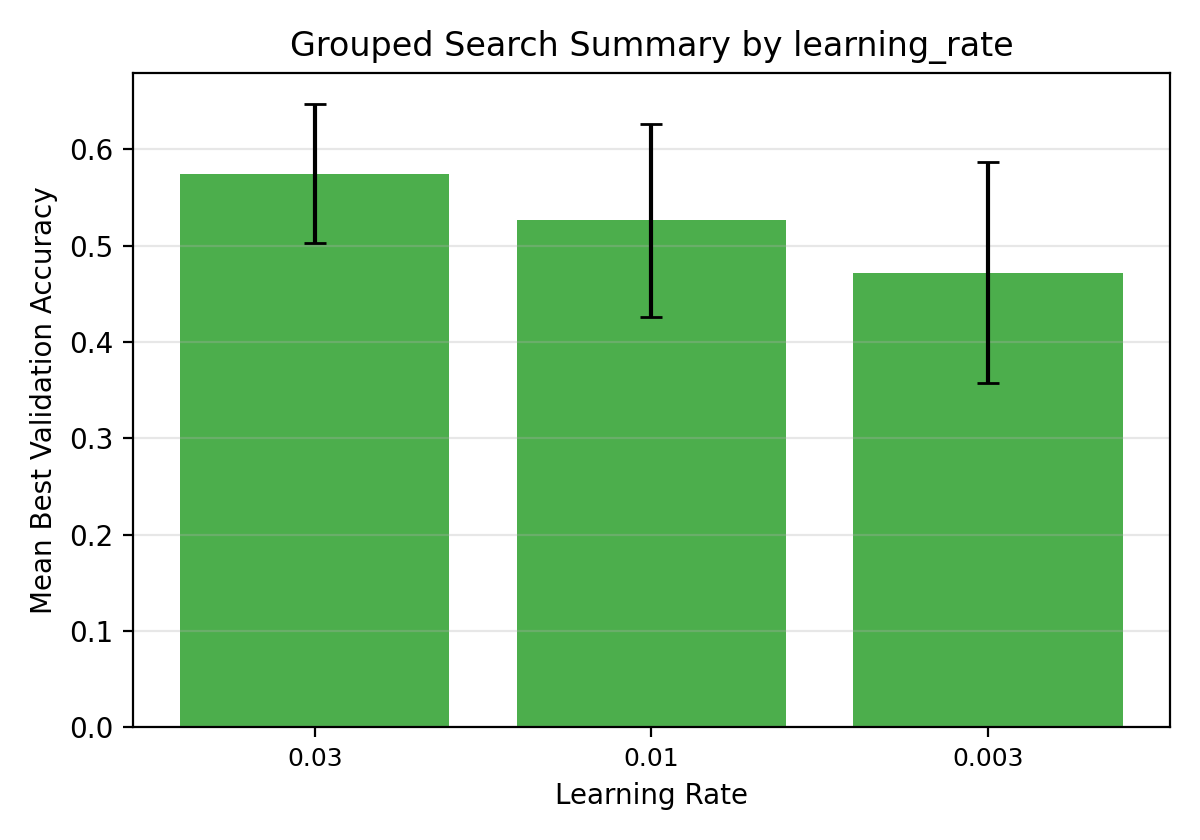
\includegraphics[width=0.49\linewidth]{../results/search/full_run_coarse_search_groupby_learning_rate.png}
  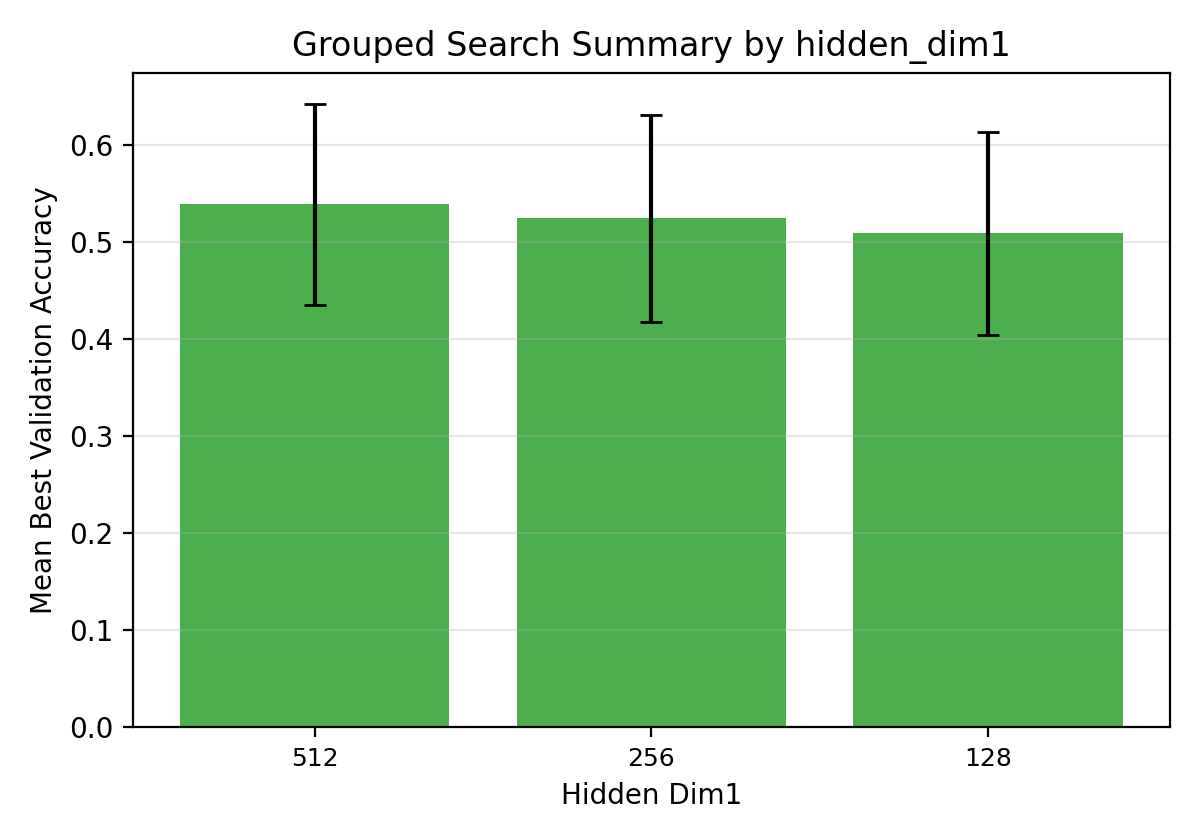
\includegraphics[width=0.49\linewidth]{../results/search/full_run_coarse_search_groupby_hidden_dim1.png}
  \caption{Grouped coarse-search statistics. The left panel shows that \(0.03\) is the strongest learning rate among the coarse candidates, while the right panel shows that larger hidden dimensions consistently improve validation accuracy.}
  \label{fig:grouped_search}
\end{figure}

\begin{figure}[ht]
  \centering
  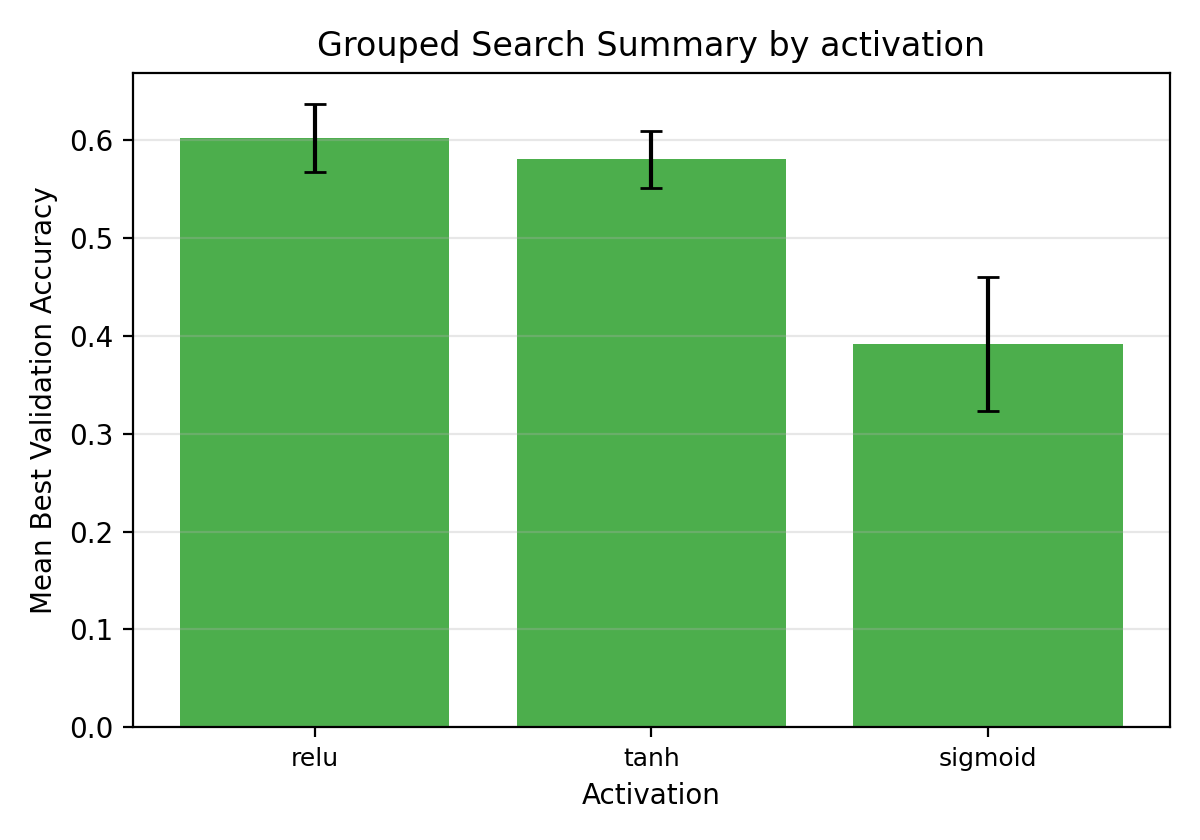
\includegraphics[width=0.49\linewidth]{../results/search/full_run_coarse_search_groupby_activation.png}
  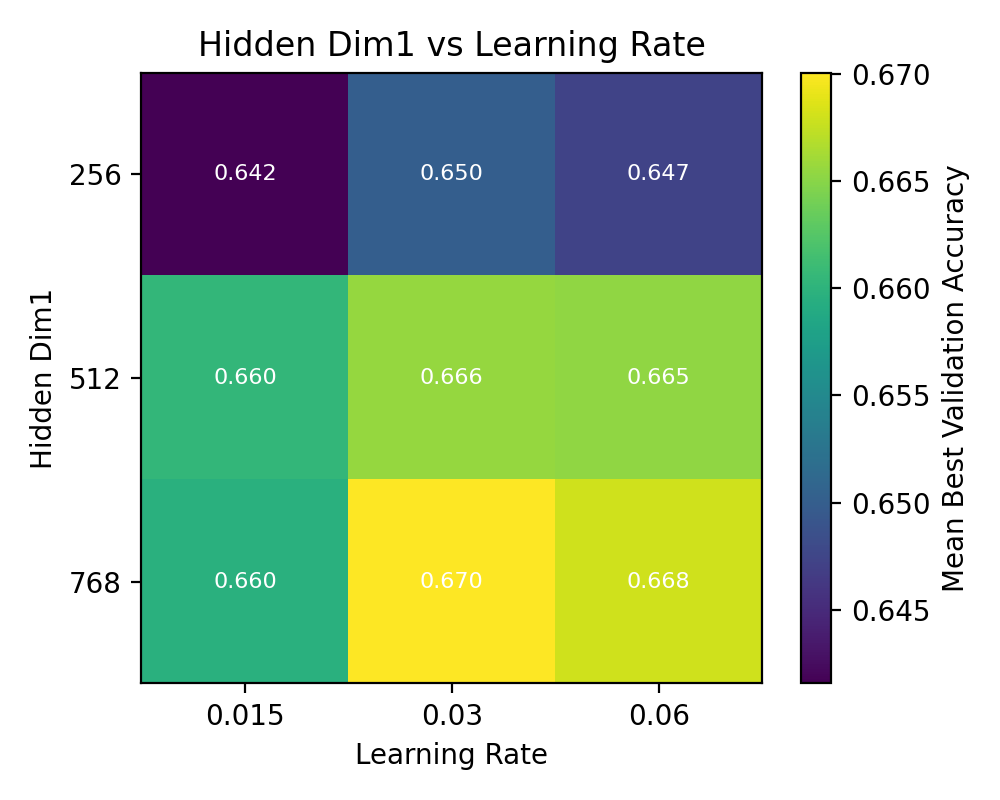
\includegraphics[width=0.49\linewidth]{../results/search/full_run_fine_search_heatmap_lr_hidden.png}
  \caption{Additional evidence from the hyperparameter study. The left panel shows the coarse-search comparison among ReLU, Tanh, and Sigmoid, where ReLU performs best and Sigmoid is clearly weakest on average. The right panel is the fine-search heatmap over learning rate and first-layer hidden width, showing that wider models combined with learning rates around \(0.03\) to \(0.06\) are consistently strong.}
  \label{fig:search_heatmaps}
\end{figure}

\section{Experimental Results}

\subsection{Validation and Test Performance}

After selecting the best configuration through the two-stage hyperparameter search, the model was trained for a final 30-epoch run and then evaluated on the held-out test set. This final experiment achieved a best validation accuracy of 0.6788 and a final test accuracy of 0.6780, as recorded in \texttt{results/curves/full\_run\_history.json} and \texttt{results/errors/full\_run\_test\_summary.json}. These values are higher than the earlier single-stage run and confirm that the search-first strategy improves the final performance of the from-scratch MLP.

The final model used the best fine-search configuration:
\begin{itemize}
\item learning rate: 0.06
\item hidden dimensions: 768 and 384
\item weight decay: \(10^{-5}\)
\item activation: ReLU
\item training epochs: 30
\end{itemize}

\begin{table}[ht]
  \caption{Final experiment summary from the completed two-stage pipeline.}
  \label{tab:final_metrics}
  \centering
  \small
  \begin{tabular}{ll}
    \toprule
    Item & Value \\
    \midrule
    Coarse search trials & 54 \\
    Fine search trials & 27 \\
    Final training epochs & 30 \\
    Best validation accuracy & 0.6788 \\
    Best validation epoch & 30 \\
    Test accuracy & 0.6780 \\
    Best final configuration & LR \(= 0.06\), hidden \(= 768/384\), WD \(= 10^{-5}\), ReLU \\
    \bottomrule
  \end{tabular}
\end{table}

Figure~\ref{fig:curves} shows the corresponding training dynamics for this final run. Training loss decreased from 1.7484 to 0.2422, while validation accuracy improved from 0.4778 to 0.6788. The best validation epoch occurred at the end of training, which suggests that the chosen schedule was still productive and did not yet exhibit a severe performance drop due to overfitting.

\begin{figure}[ht]
  \centering
  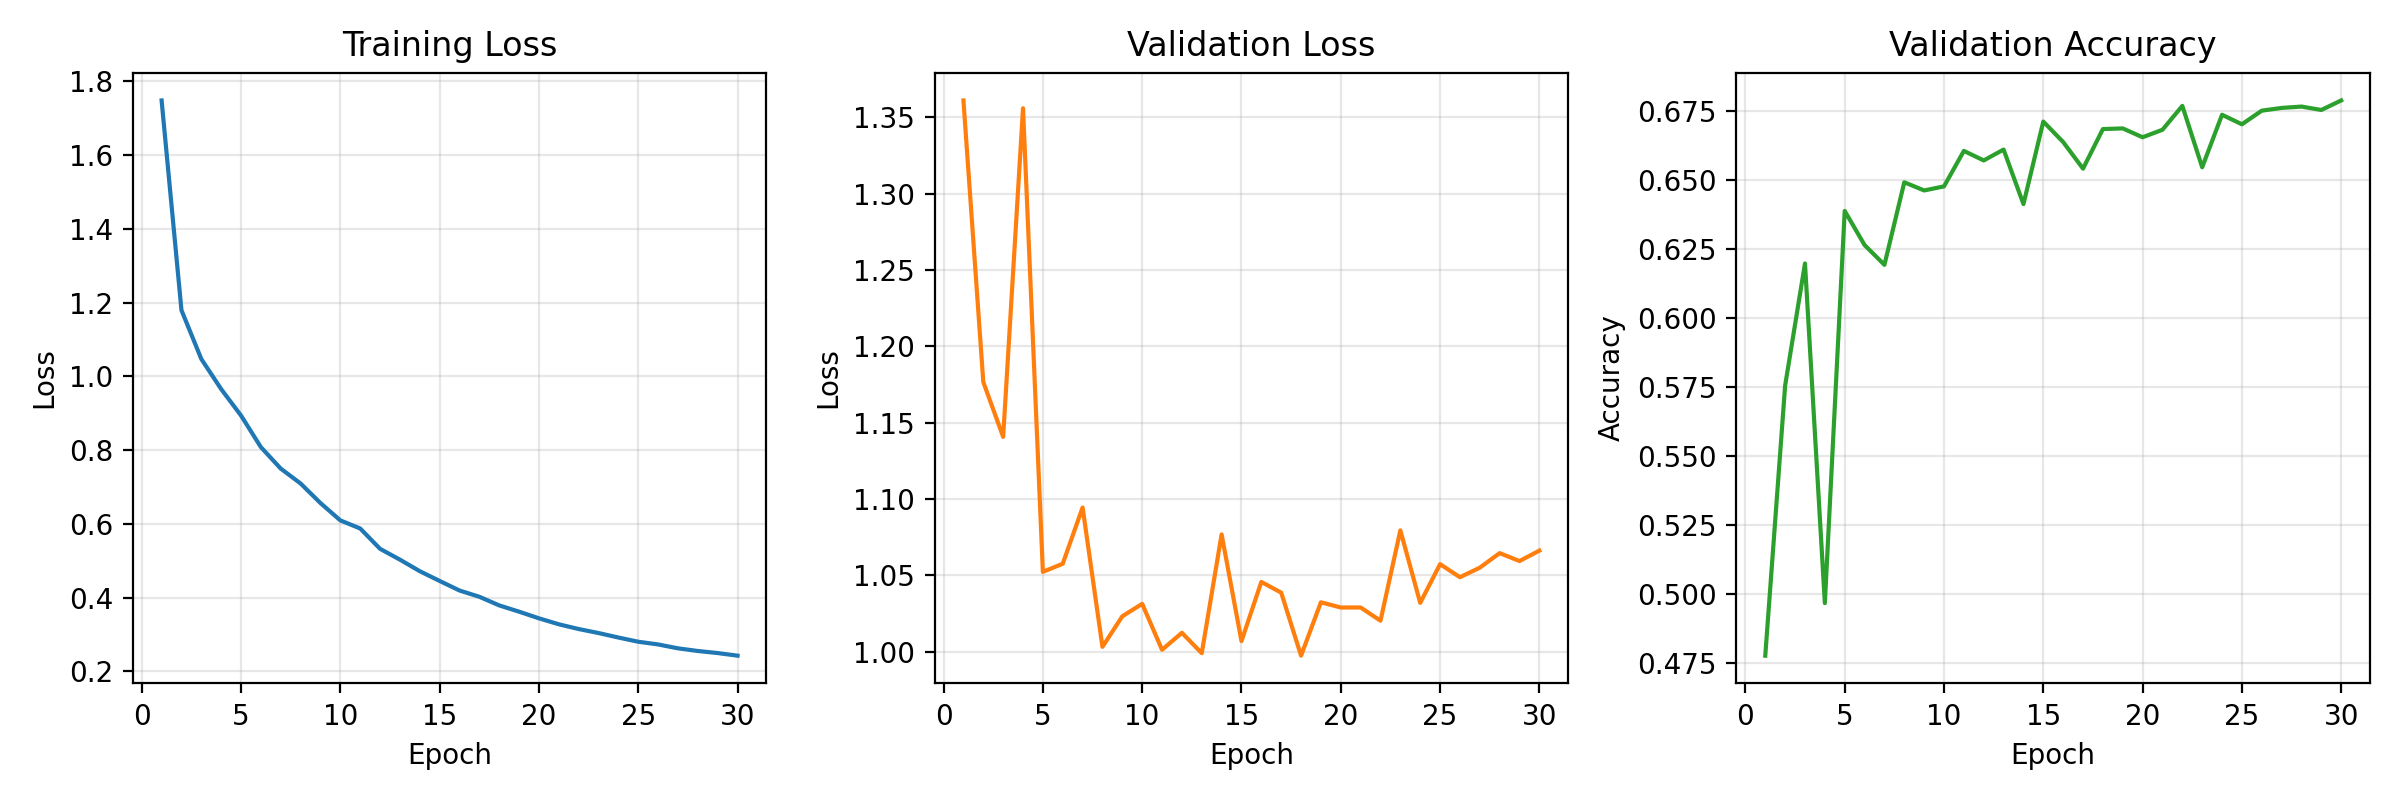
\includegraphics[width=\linewidth]{../results/curves/full_run_curves.png}
  \caption{Training loss, validation loss, and validation accuracy for the final 30-epoch run after hyperparameter selection. The validation accuracy improves steadily and reaches its best value at the end of training.}
  \label{fig:curves}
\end{figure}

The confusion matrix in Figure~\ref{fig:confusion} provides a more detailed class-wise view. Some classes are recognized relatively well:
\begin{itemize}
\item Industrial: 0.8347 class accuracy
\item Forest: 0.7956 class accuracy
\item SeaLake: 0.8333 class accuracy
\item Pasture: 0.7700 class accuracy
\item Residential: 0.7022 class accuracy
\item River: 0.6853 class accuracy
\end{itemize}

However, other categories remain difficult:
\begin{itemize}
\item Highway: 0.4027 class accuracy
\item HerbaceousVegetation: 0.5178 class accuracy
\item PermanentCrop: 0.5947 class accuracy
\end{itemize}

\begin{figure}[ht]
  \centering
  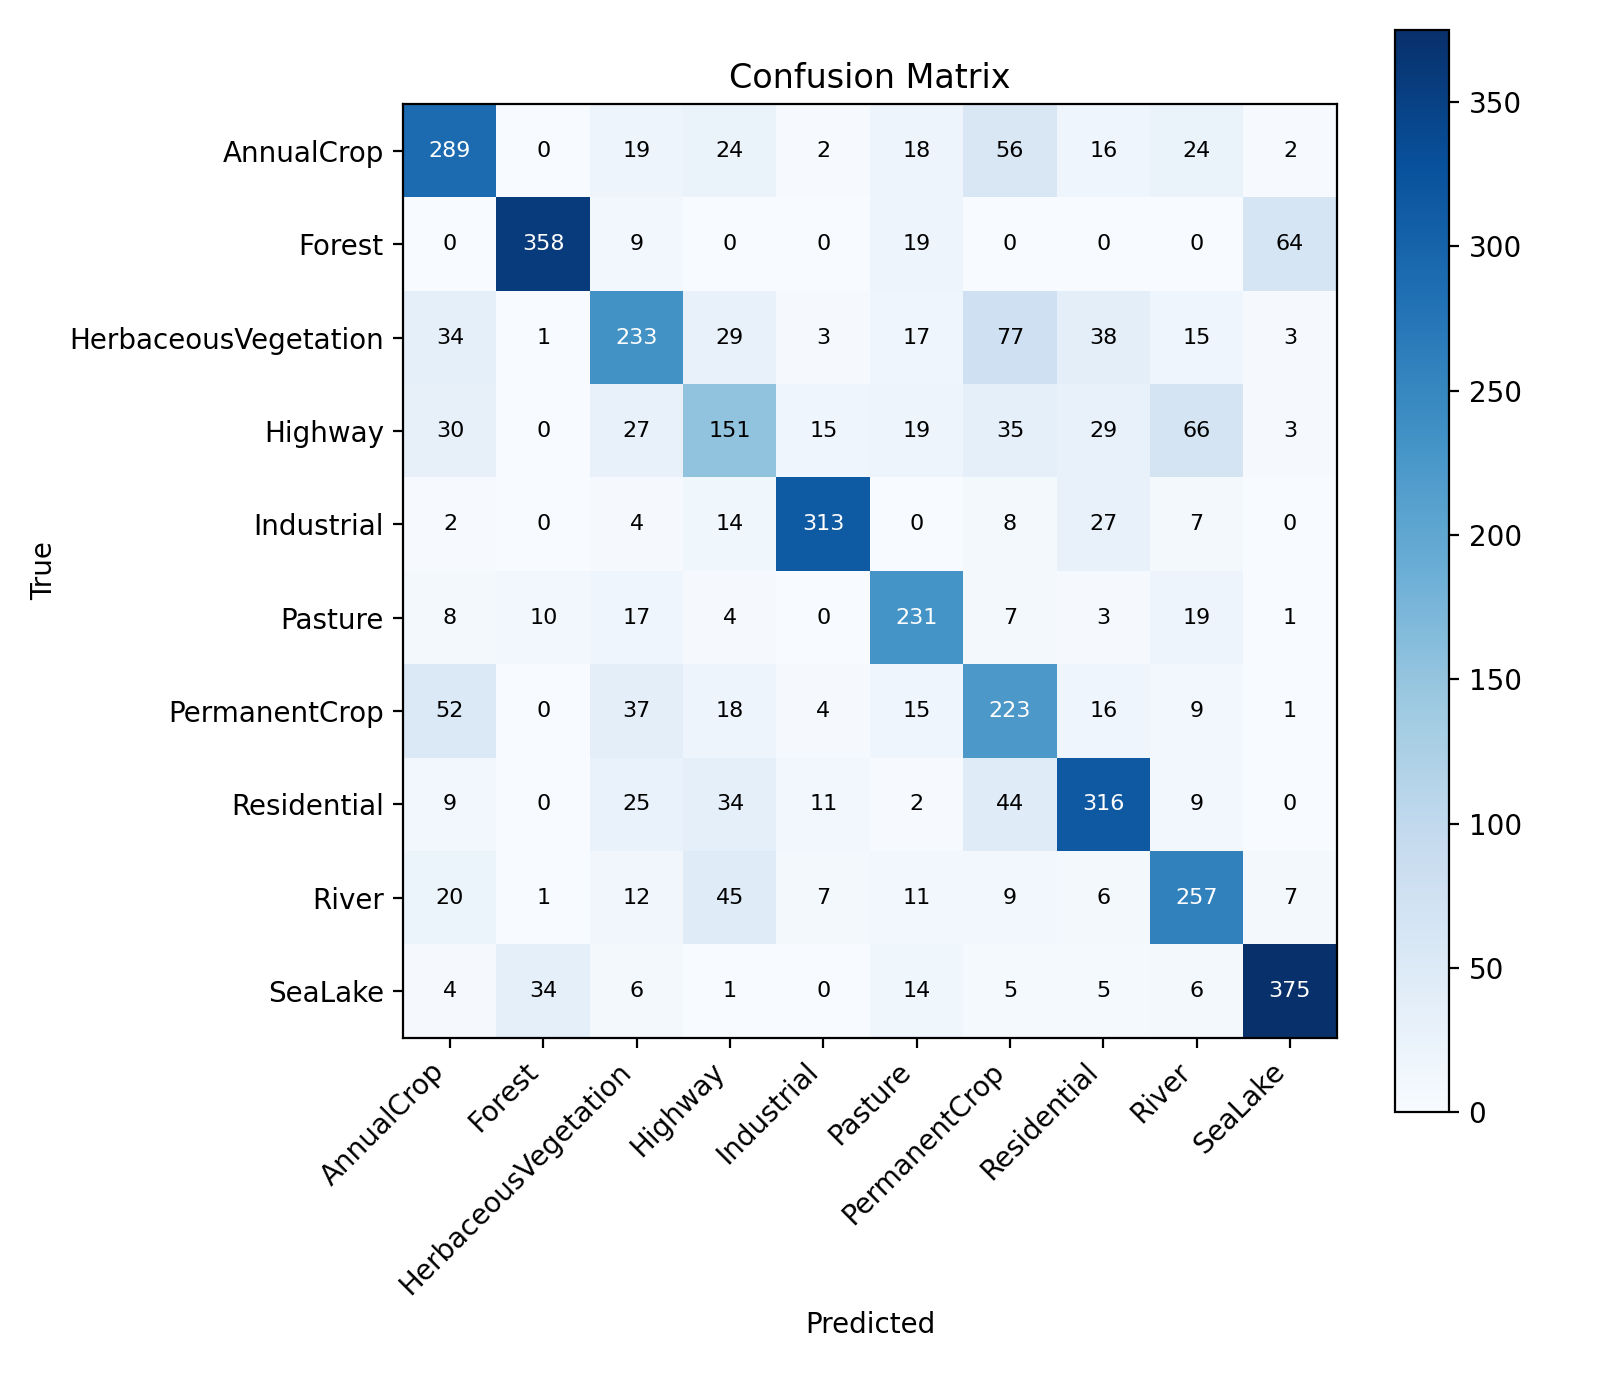
\includegraphics[width=0.82\linewidth]{../results/errors/full_run_test_confusion_matrix.png}
  \caption{Confusion matrix on the test set for the final 30-epoch run. Strong diagonal entries indicate correct predictions, while off-diagonal mass highlights systematic class confusions.}
  \label{fig:confusion}
\end{figure}

Several confusion patterns are especially noticeable. Highway is still frequently confused with River and Residential, although its class accuracy improves relative to the earlier run. PermanentCrop remains strongly entangled with AnnualCrop and HerbaceousVegetation, which reflects the visual similarity of agricultural texture and vegetation distribution. Forest and SeaLake are both strong classes overall, but Forest is still occasionally confused with SeaLake in images dominated by large, dark, low-texture regions.

\subsection{First-Layer Weight Visualization}

The first-layer weight visualization is included in Appendix~\ref{app:extra_figures}. The weights were reshaped back to the spatial image size for qualitative inspection. Compared with convolutional filters, these patterns are much less interpretable. Most units show diffuse color-sensitive mosaics rather than crisp localized edges or object-part templates.

This behavior is consistent with the architecture. Because the model is a fully connected MLP operating on flattened pixels, it does not preserve local spatial neighborhoods in the same way as a convolutional network. Even so, the weight maps are not completely structureless: several units exhibit weak preferences for greenish vegetation tones, bluish water-like tones, and brown-gray man-made surfaces. This suggests that the first layer has learned coarse global color and texture cues, although the representation is still limited in spatial specificity.

\subsection{Error Analysis}

Representative misclassified test samples are included in Appendix~\ref{app:extra_figures}. The selected examples match the confusion-matrix trends and reveal several recurring failure modes.

First, linear structures create ambiguity among Highway, River, and Residential. In multiple examples, a wide road corridor or road-like strip is predicted as River, while dense urban or industrial layouts are sometimes predicted as Highway or Residential. This indicates that the MLP is sensitive to coarse global geometry but does not robustly distinguish material type or surrounding context.

Second, agricultural classes are visually entangled. AnnualCrop, PermanentCrop, HerbaceousVegetation, and Pasture often share repetitive field textures, similar color tones, and large homogeneous regions. When the image is flattened, the model must rely on global appearance rather than local arrangement, which makes these categories particularly difficult to separate.

Third, dark and homogeneous images can also be confusing. For example, SeaLake and Forest can both contain large low-texture regions, and some Forest images are misclassified as Pasture or HerbaceousVegetation when canopy texture is weak.

Overall, the error cases suggest that the model has learned more robust global representations than in the earlier baseline, but it still lacks an explicit mechanism for modeling translation-invariant local structure. This limitation is expected for a dense MLP on remote-sensing imagery and explains why semantically related classes remain hard to distinguish even after careful hyperparameter tuning.

\section{Conclusion}

This homework implemented a complete three-layer MLP classifier for EuroSAT RGB classification using only NumPy and manual backpropagation. The project covers the full pipeline required by the assignment: data loading, preprocessing, model definition, loss computation, SGD optimization, learning-rate decay, weight decay, checkpoint saving, staged hyperparameter search, testing, and visualization.

The final experiment used a clear strategy: broad coarse search, focused fine search, and then full training with the best refined configuration. This strategy raised the final validation accuracy to 0.6788 and the test accuracy to 0.6780, which improves on the earlier baseline and provides a more convincing experimental study for the report.

From the completed experiments, three main conclusions are supported by the data. First, a staged hyperparameter search is worthwhile even for a homework-scale MLP: the final system improved over the earlier baseline because search was treated as a real experiment instead of a small appendix. Second, model width and learning rate matter more than small changes in weight decay within the tested range, and the coarse activation comparison shows that Sigmoid is notably less suitable than ReLU or Tanh for this optimization setting. Third, the remaining errors are not random; they mostly reflect visually similar remote-sensing categories that are difficult for a fully connected model operating on flattened pixels.

The main strengths of the project are the correctness of the from-scratch implementation, the modular experiment pipeline, and the more complete hyperparameter study. The main weakness remains representational capacity: without convolution, the model still cannot exploit local spatial structure as effectively as a CNN. A natural extension would be to preserve the manually implemented learning framework while exploring architectures that better model local patterns or spatial inductive bias.

\section*{Reproducibility Notes}

The report text above is tied to the currently available local experiment artifacts. In particular, the cited values come from:
\begin{itemize}
\item \texttt{results/curves/full\_run\_history.json}
\item \texttt{results/errors/full\_run\_test\_summary.json}
\item \texttt{results/search/full\_run\_coarse\_search\_summary.json}
\item \texttt{results/search/full\_run\_fine\_search\_summary.json}
\item the corresponding PNG figures under \texttt{results/curves/}, \texttt{results/errors/}, \texttt{results/search/}, and \texttt{results/weights/}
\end{itemize}

\newpage
\appendix
\section{Full Search Ranking Figures}
\label{app:search_rankings}

The main text focuses on grouped statistics and interaction heatmaps because they convey the search trends more compactly. For completeness, the full per-configuration ranking plots for the coarse and fine searches are included below.

\begin{figure}[ht]
  \centering
  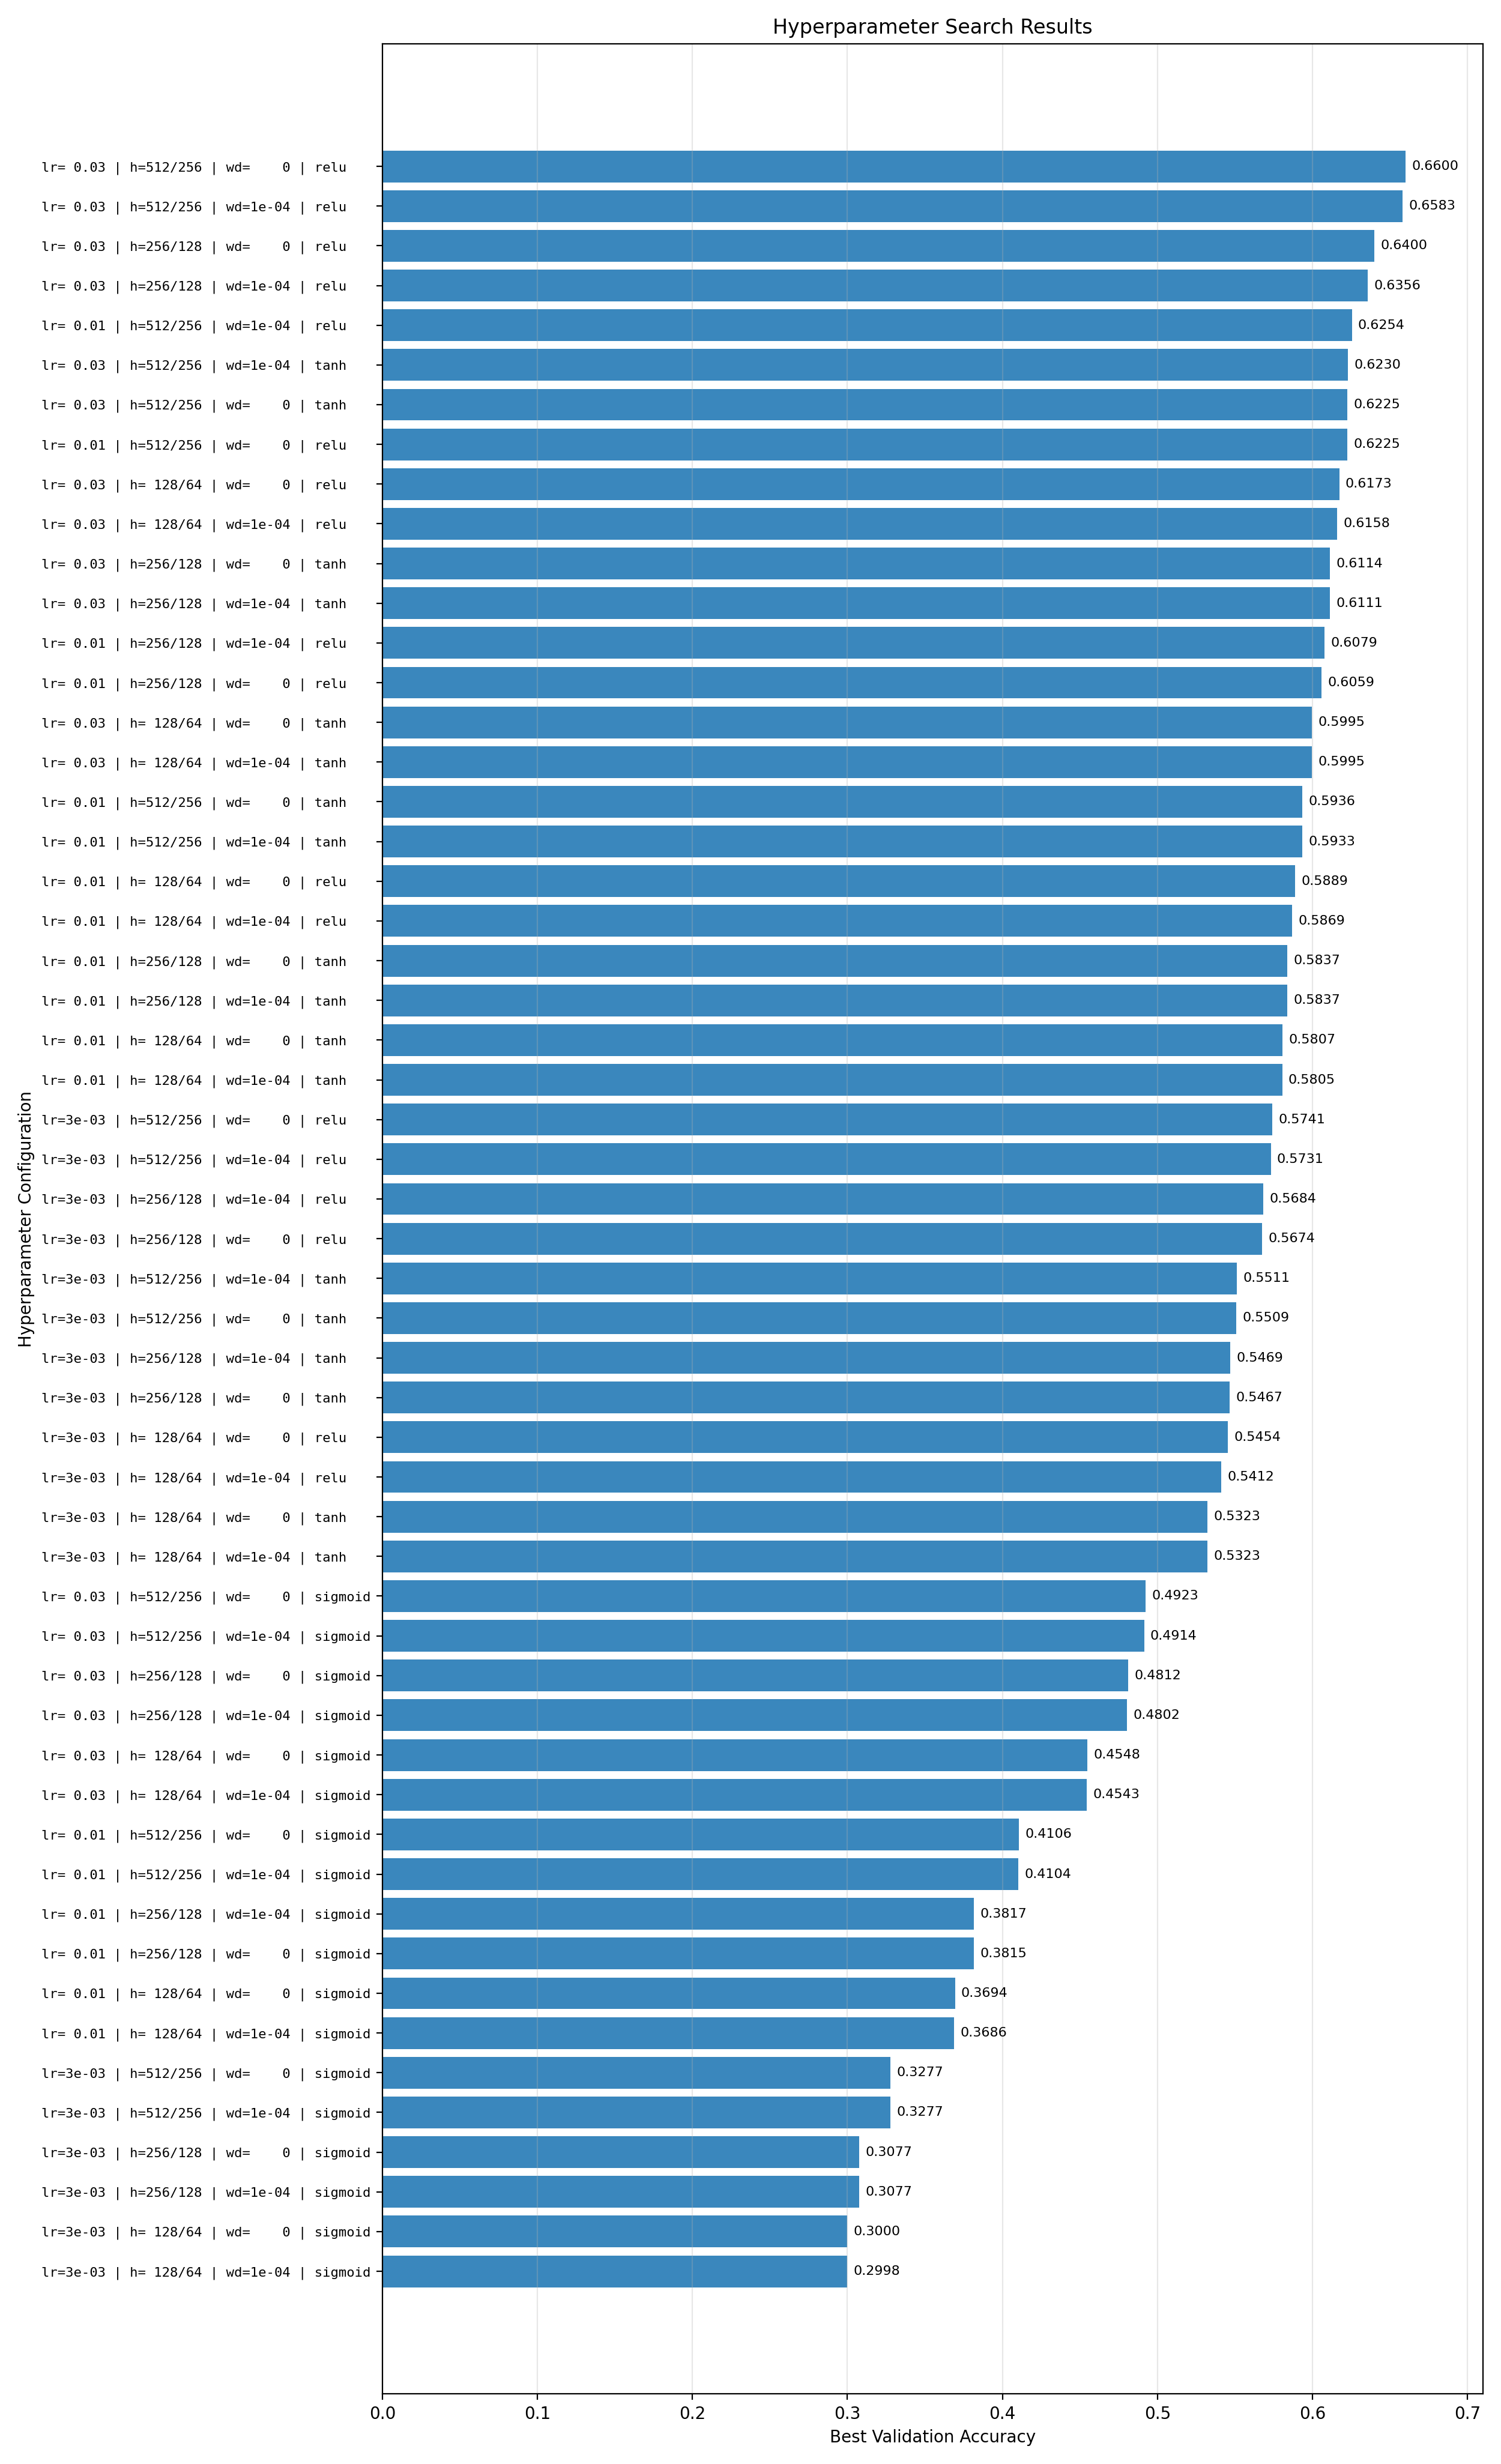
\includegraphics[width=0.80\linewidth]{../results/search/full_run_coarse_search_best_val_accuracy.png}
  \caption{Full ranking of validation accuracy for the coarse search configurations. The highest-ranked settings are dominated by ReLU, larger hidden dimensions, and learning rate \(0.03\), while Sigmoid configurations are concentrated in the lower part of the ranking.}
  \label{fig:search}
\end{figure}

\begin{figure}[ht]
  \centering
  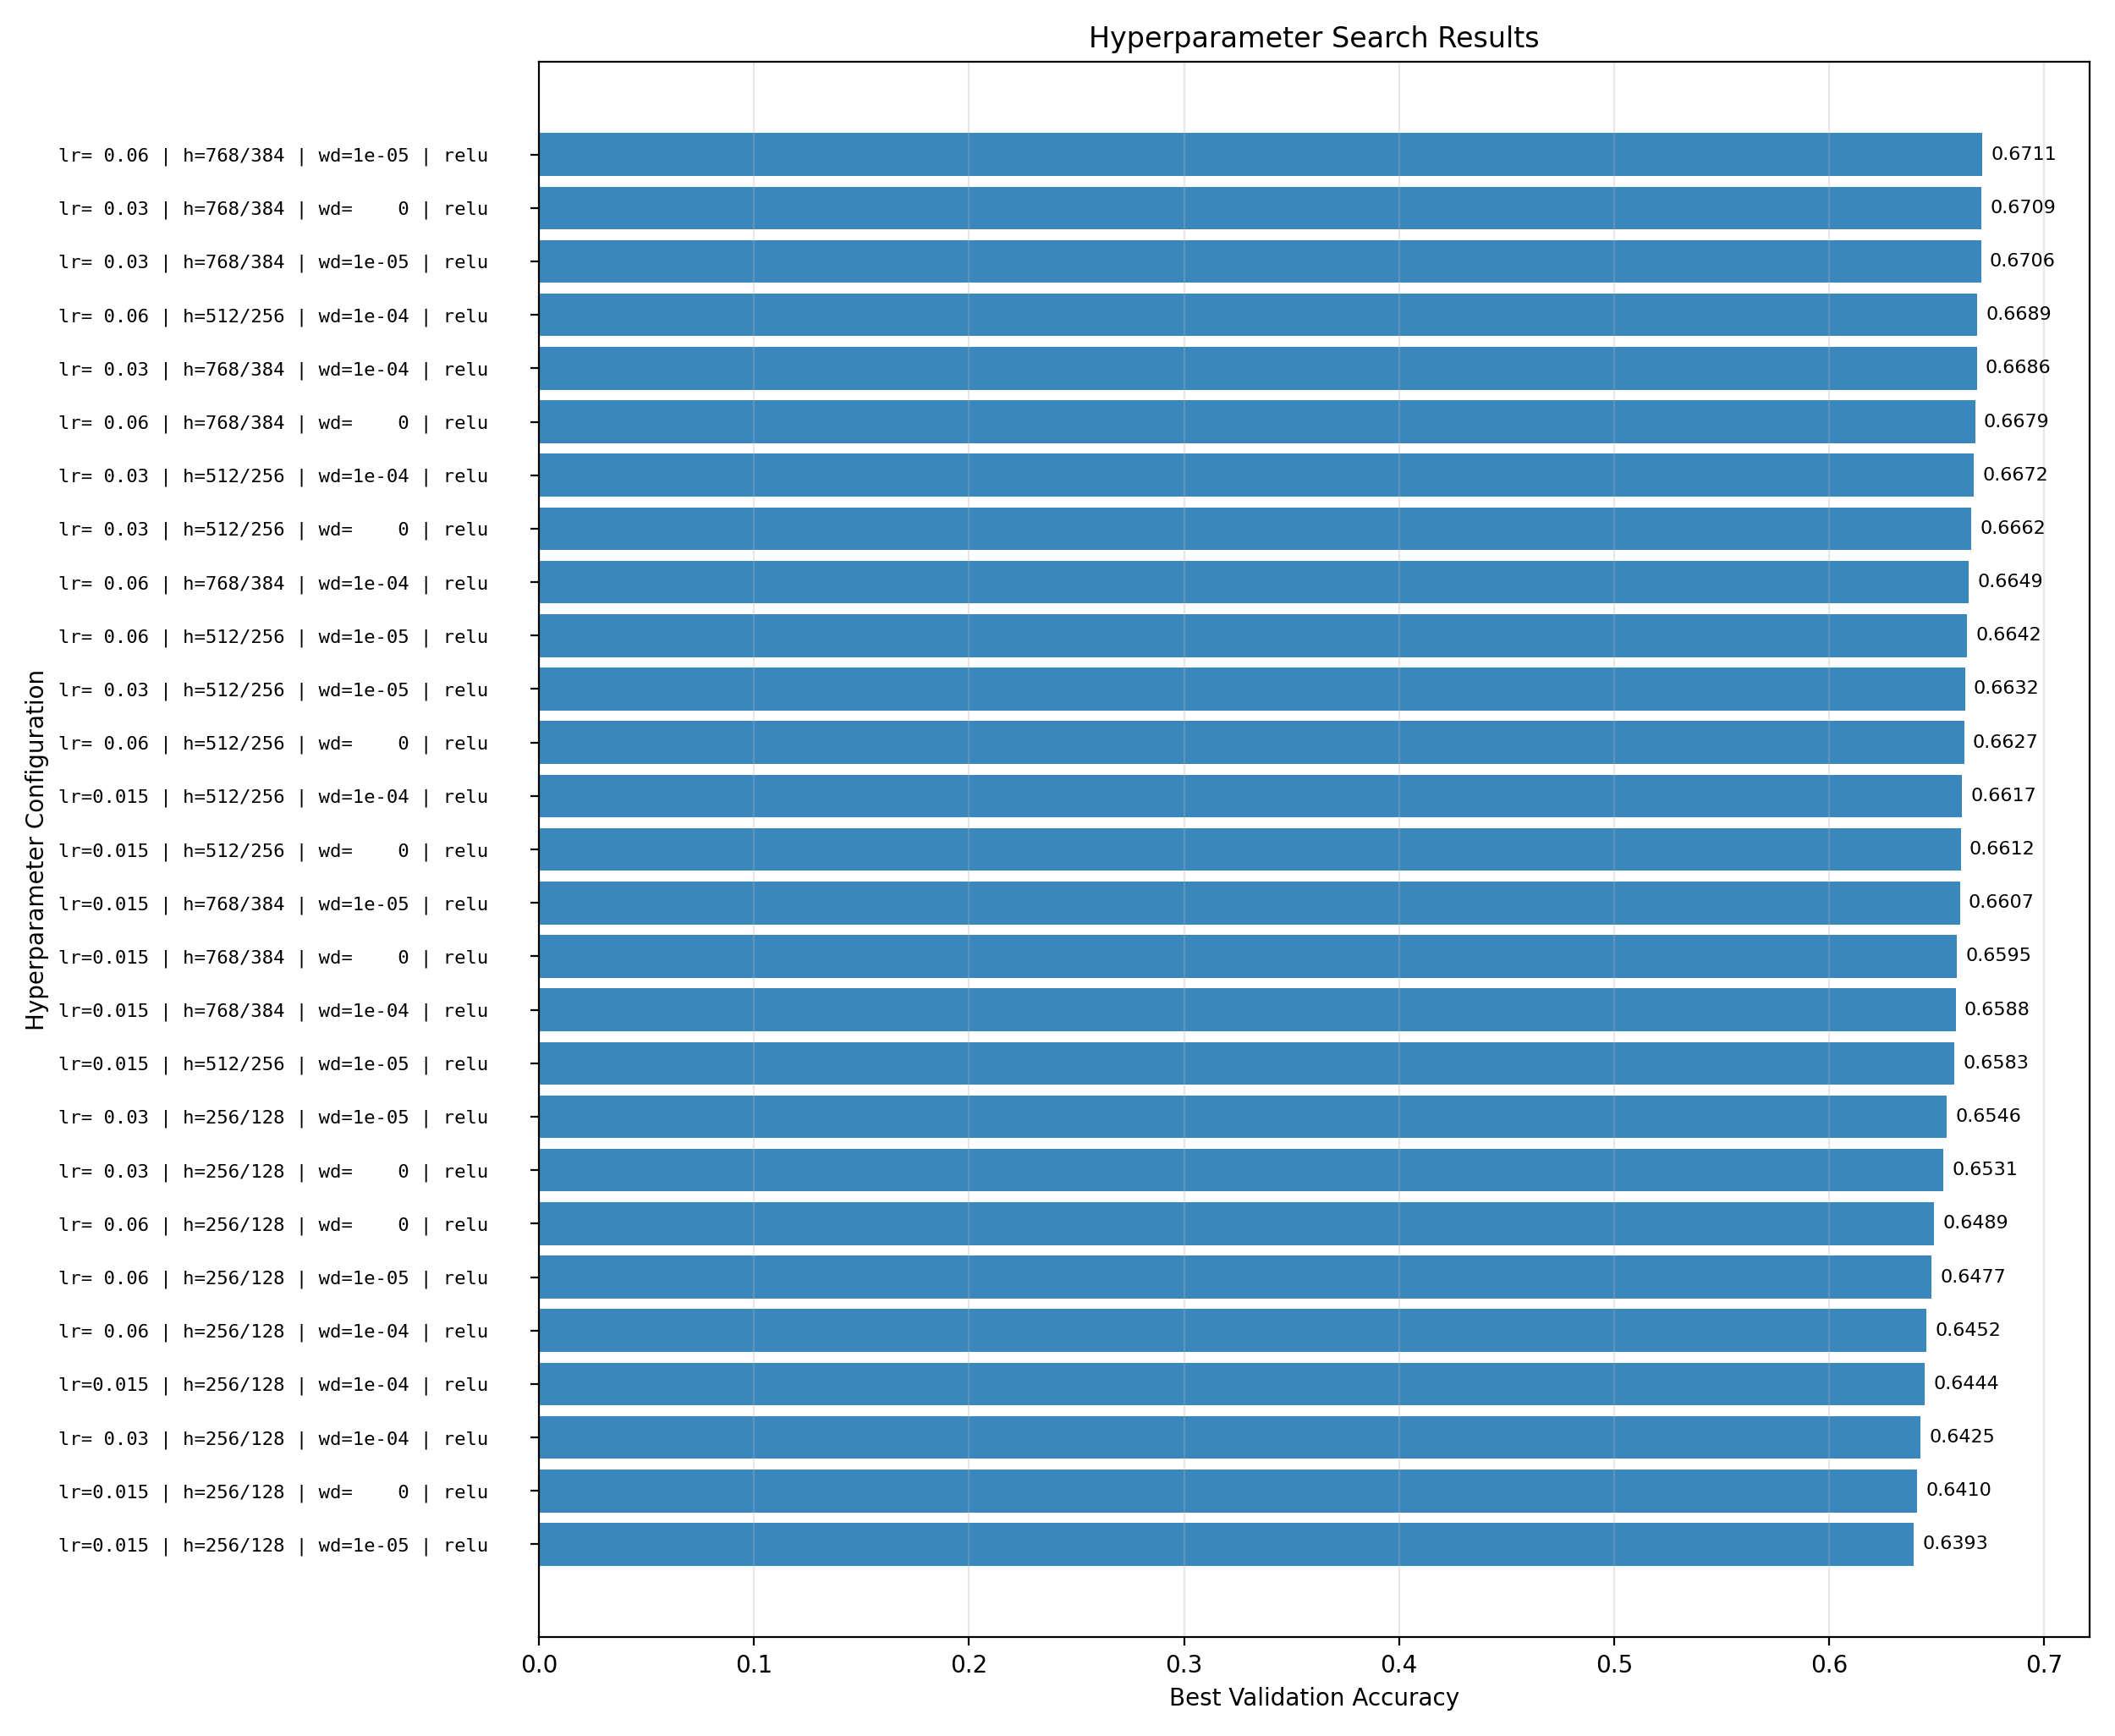
\includegraphics[width=0.82\linewidth]{../results/search/full_run_fine_search_best_val_accuracy.png}
  \caption{Full ranking of validation accuracy for the fine search configurations. The best-performing region is concentrated around hidden widths \(768/384\) and learning rates \(0.03\) to \(0.06\).}
  \label{fig:fine_search}
\end{figure}

\newpage

\section{Additional Qualitative Figure}
\label{app:extra_figures}

\begin{figure}[ht]
  \centering
  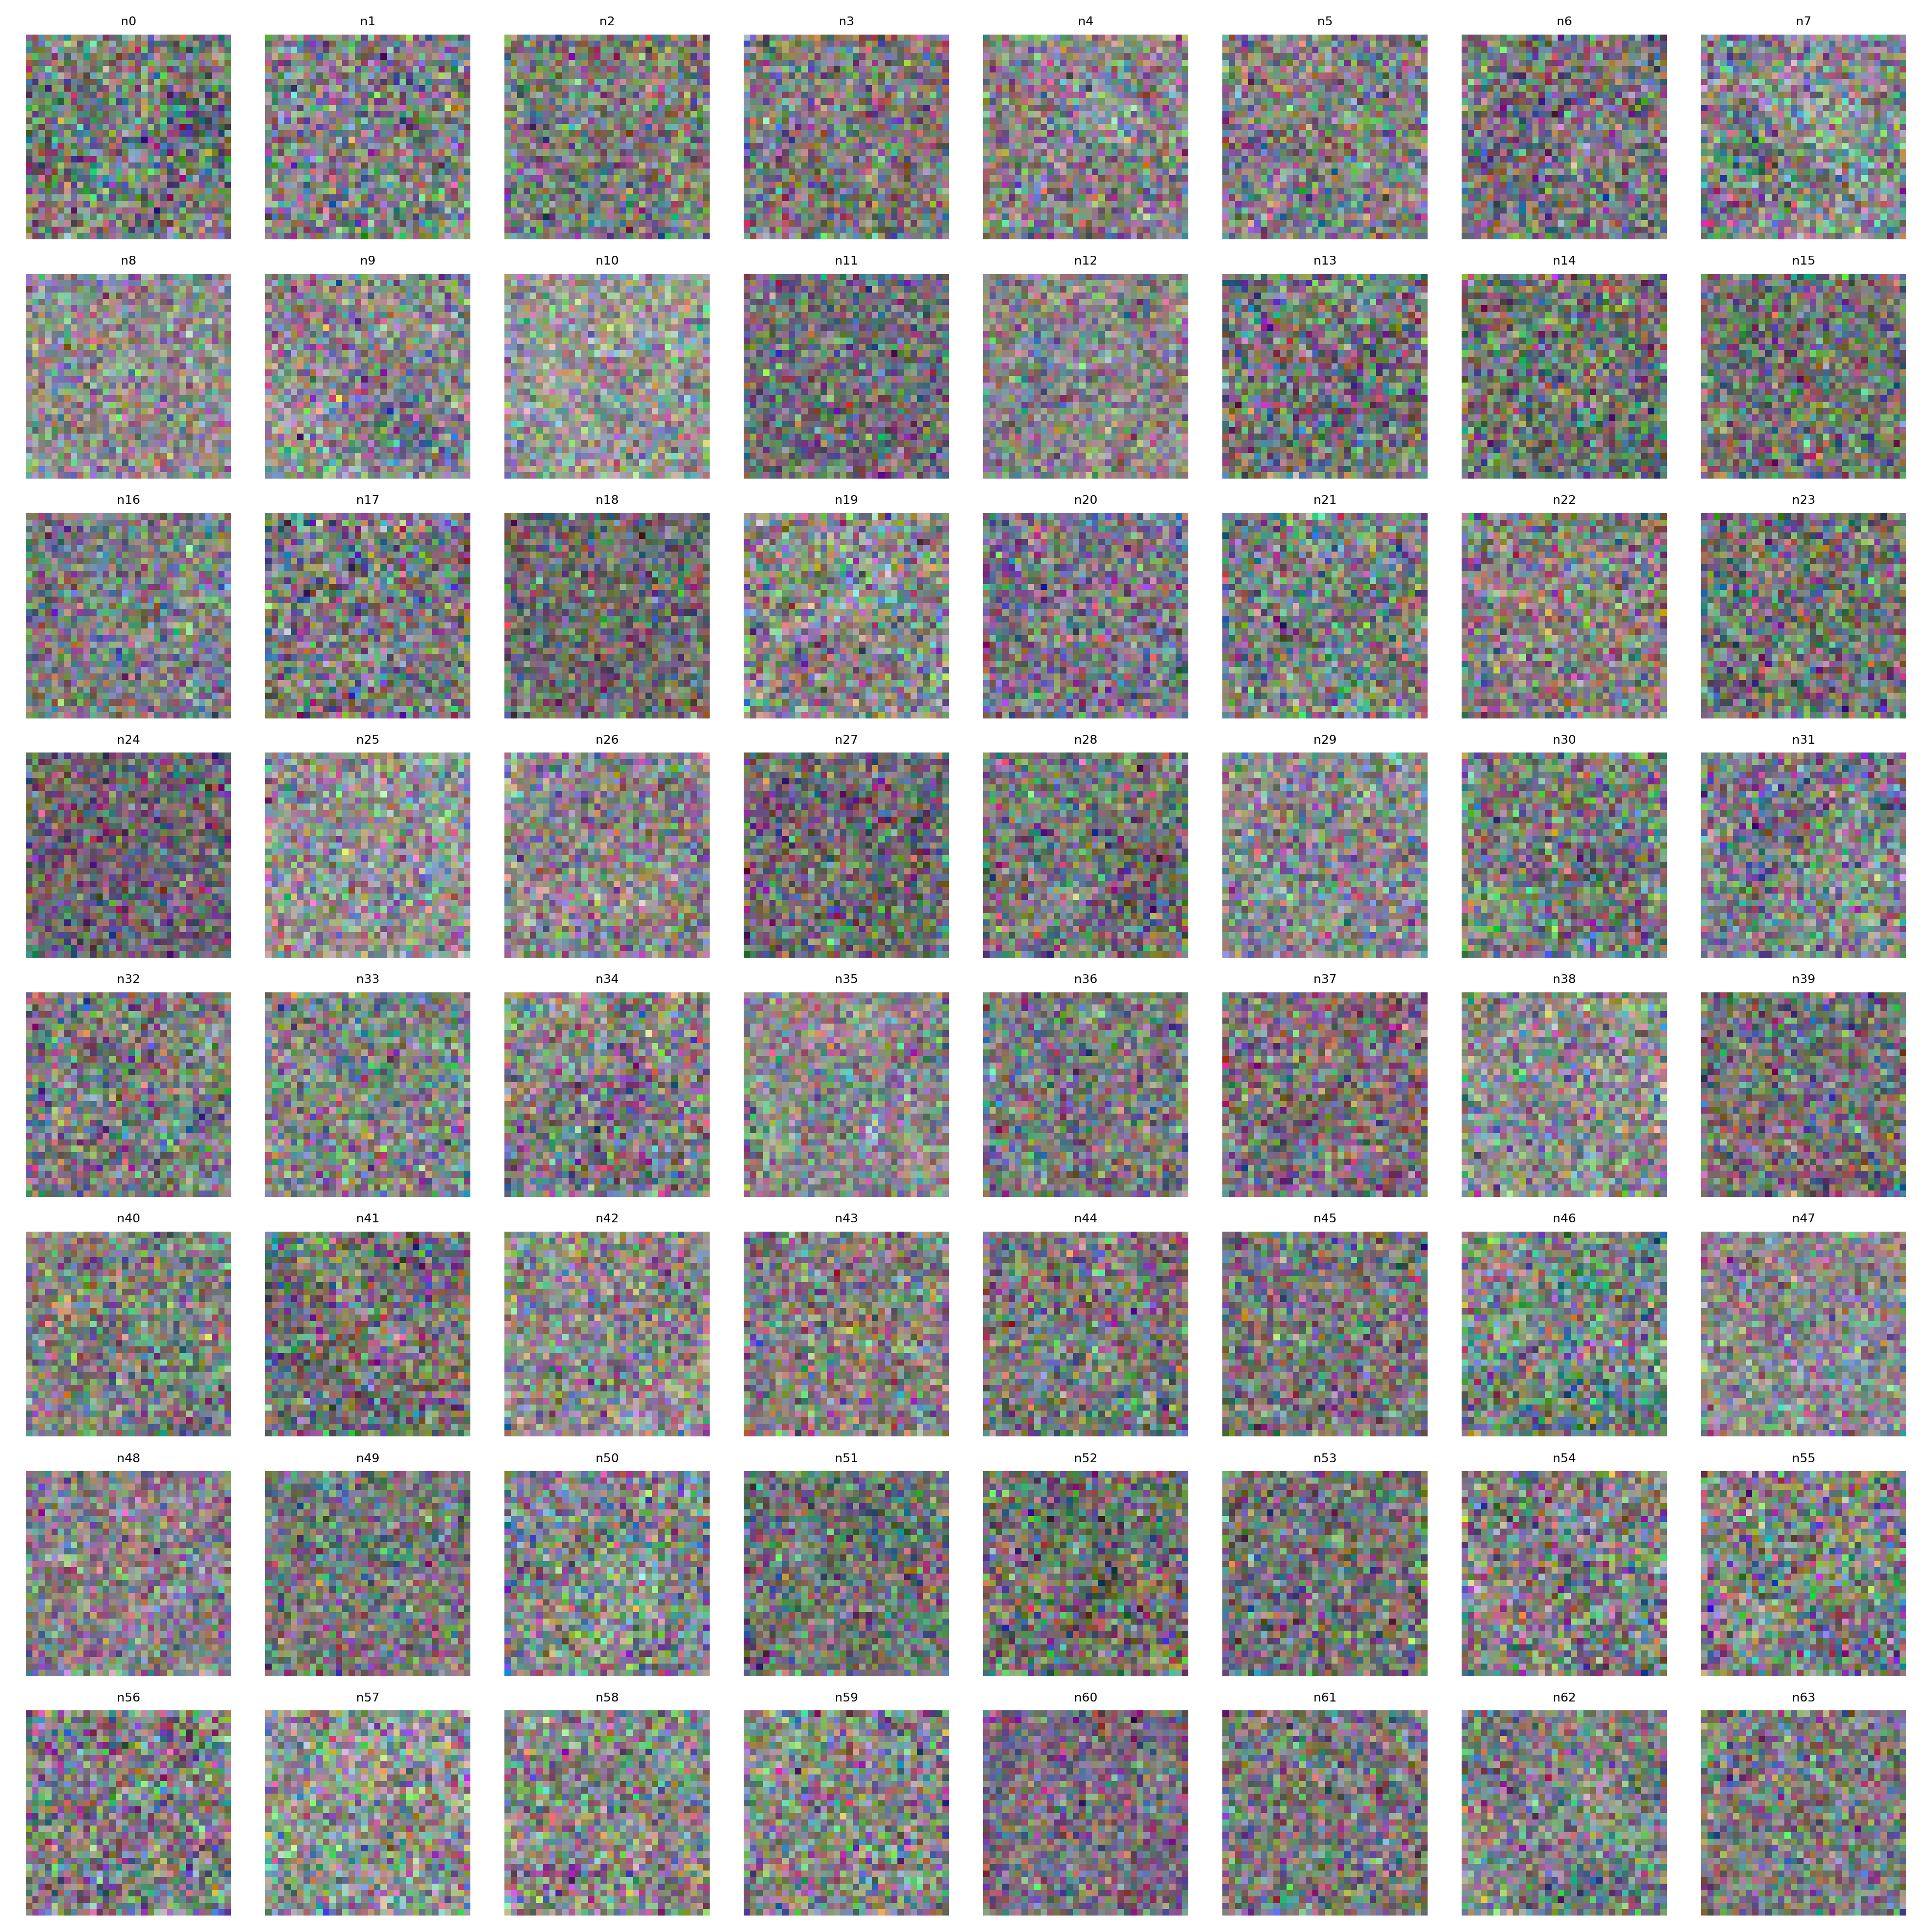
\includegraphics[width=\linewidth]{../results/weights/full_run_first_layer_weights.png}
  \caption{Visualization of first-layer weights reshaped to the input image size. The patterns are mostly coarse color-texture templates rather than sharp local filters, reflecting the limitations of a flattened MLP representation.}
  \label{fig:weights}
\end{figure}

\begin{figure}[ht]
  \centering
  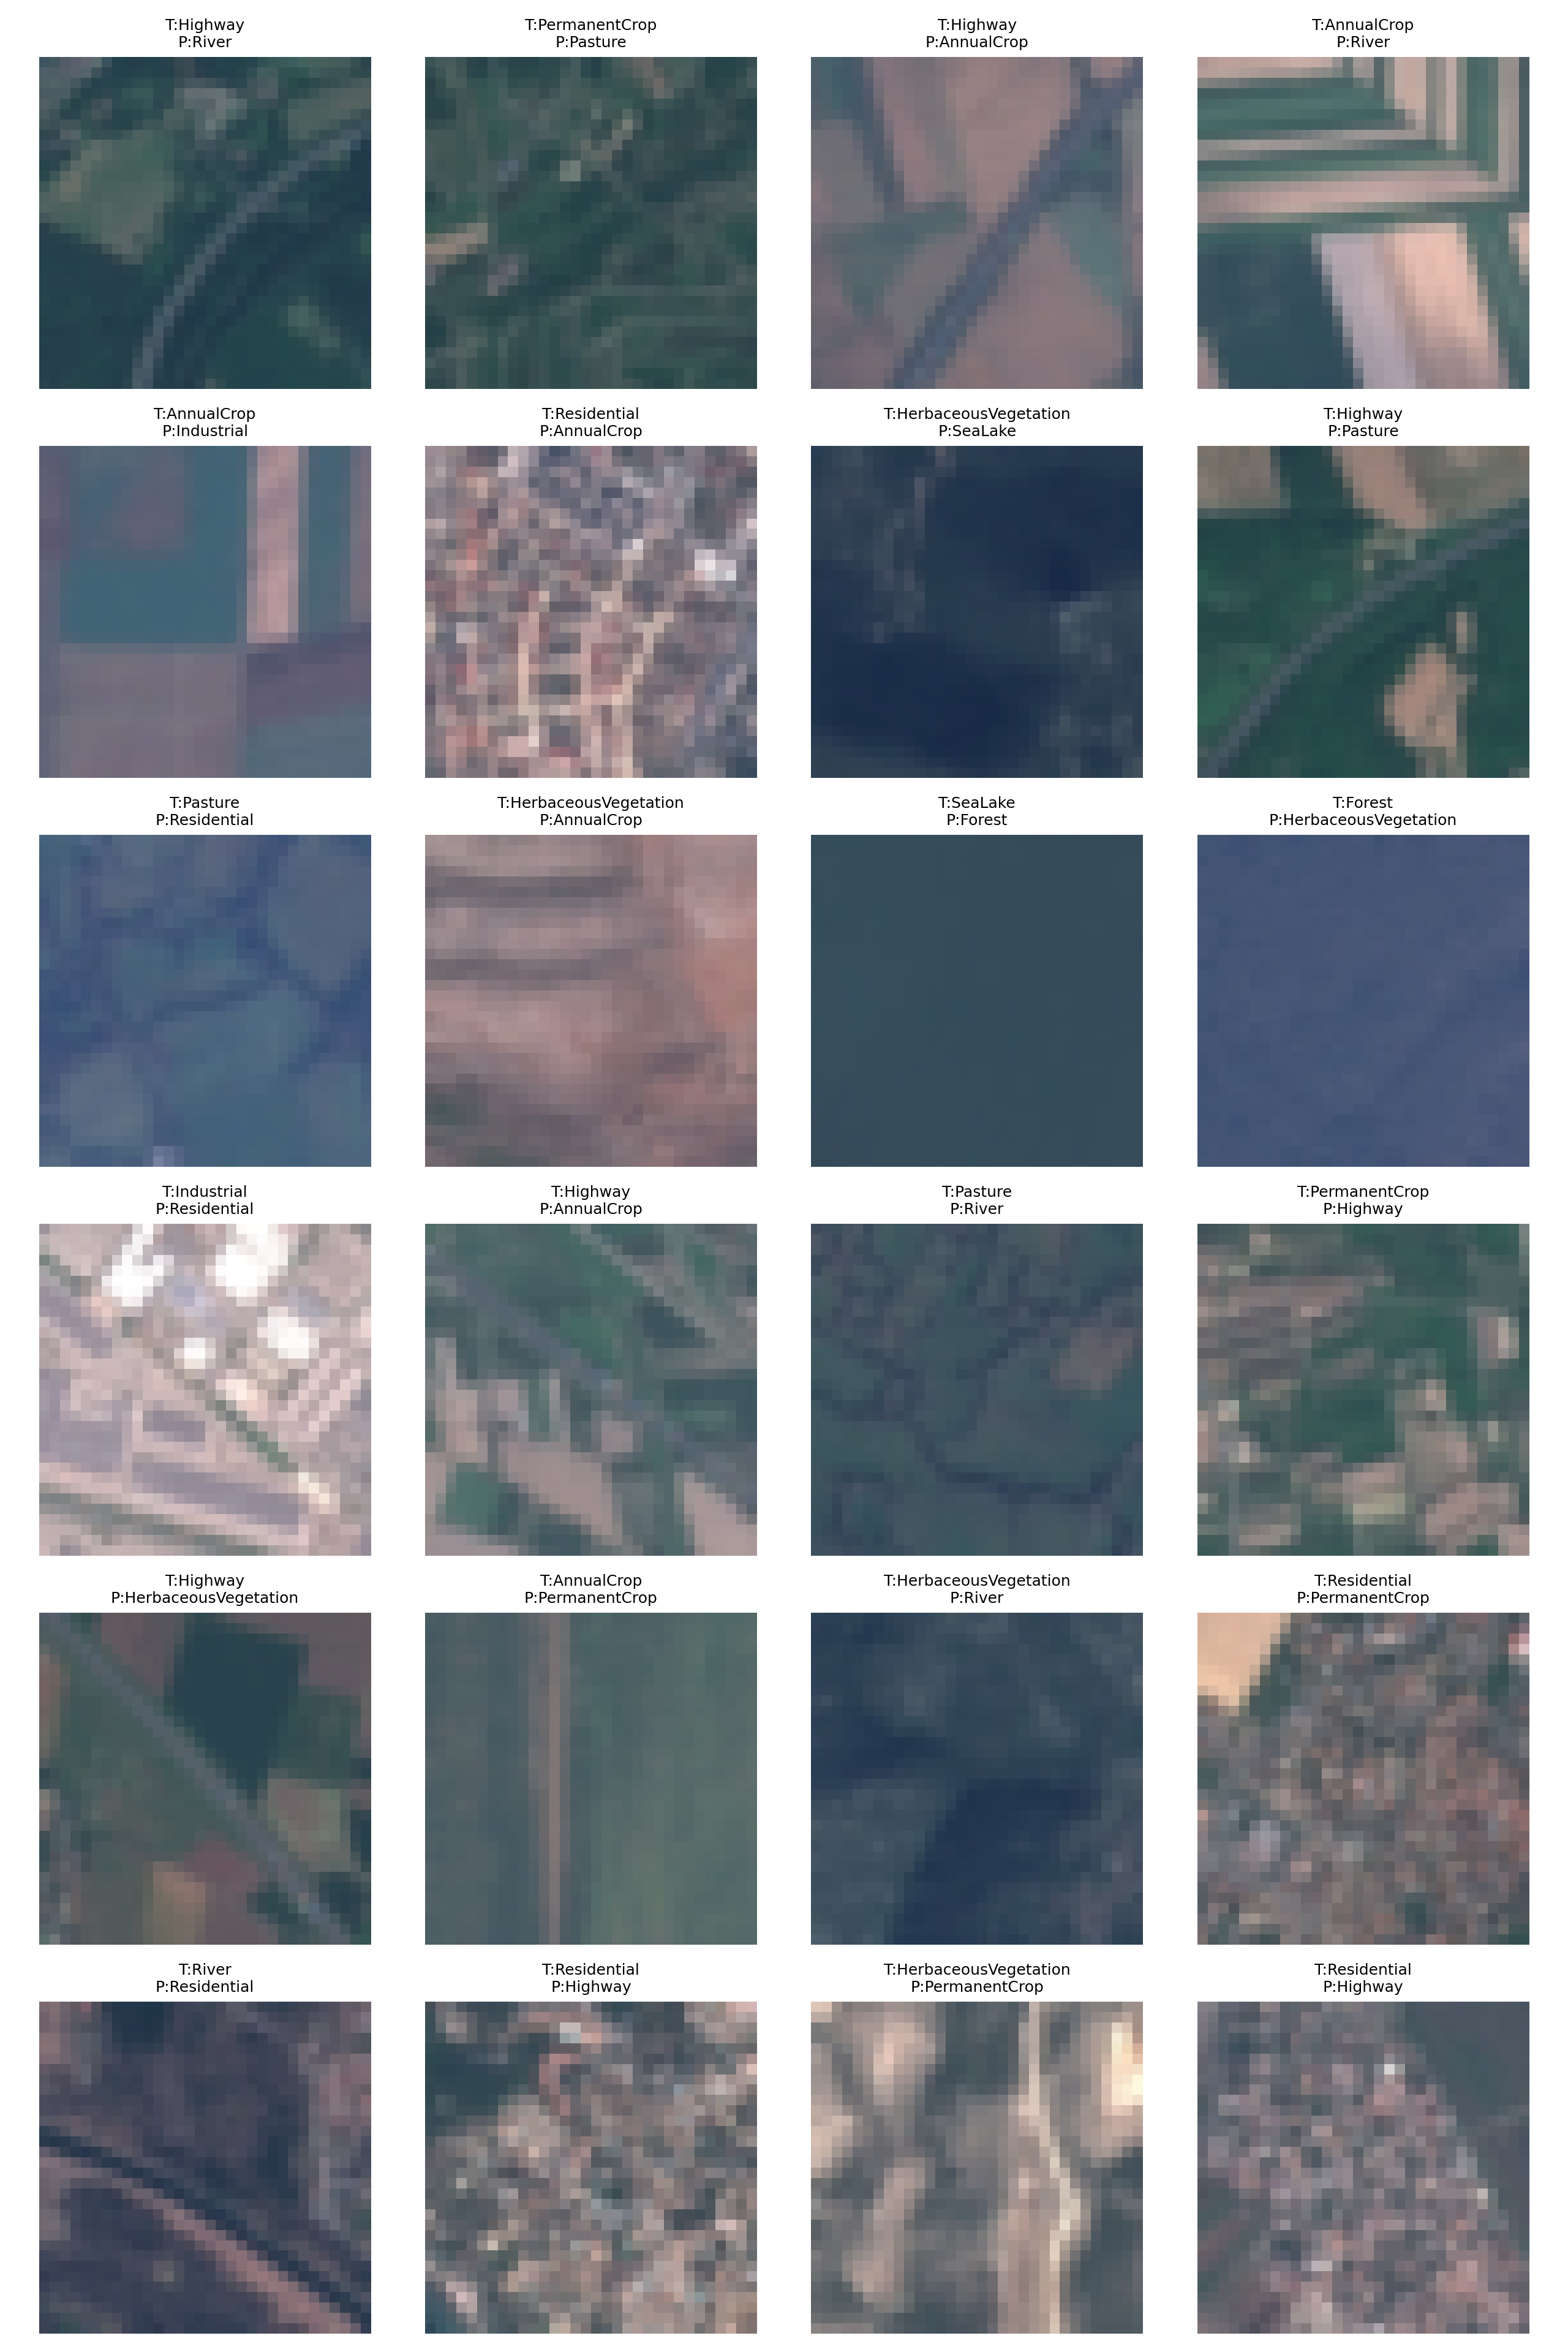
\includegraphics[width=\linewidth]{../results/errors/full_run_test_misclassified.png}
  \caption{Representative misclassified test samples. Many errors occur between visually similar land-cover categories such as Highway versus River/Residential and AnnualCrop versus PermanentCrop/HerbaceousVegetation.}
  \label{fig:errors}
\end{figure}

\end{document}
